%
% LaTeX Report Assignment 4
% Applied Programming Lab EE2703
% Ayush Jamdar EE20B018 
%


\documentclass[11pt, a4paper]{article}
\usepackage{graphicx}
\usepackage{amsmath}
\usepackage{listings}
\usepackage[]{courier}
%\usepackage{hyperref}


\title{Assignment 7: Circuit Analysis Using Sympy} % Title

\author{Ayush Jamdar EE20B018} % Author name

\date{\today} % Date for the report
\begin{document}		
		
\maketitle % Insert the title, author and date
\section{Aim}
The goal of this assignment is to learn and apply two powerful capabilities of Python - Symbolic Algebra and Circuit analysis using Laplace transforms.

\section{Introduction: A Circuit Analysis}
To get a hang of sympy and recall the use of the \texttt{scipy.signal} toolkit, we start by analysing a Low Pass Filter realised with an active RC circuit shown in Figure 1. 
 
  \begin{figure}[!tbh]
   	\centering
  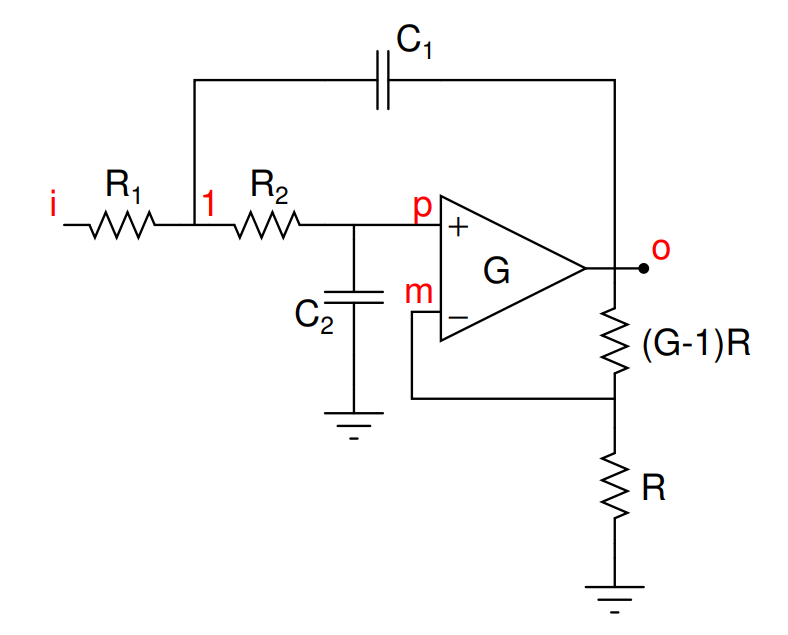
\includegraphics[scale=0.5]{lpfckt.png} 
    \caption{Low Pass Filter Circuit} 	
    %\label{time response q3.5}
   \end{figure} 
   
Using KVL,  we get

\begin{equation}
\centering
	 V_m = V_o/G  
\end{equation}

\begin{equation}
\centering
	 V_p = V_1(\frac{1}{1+j \omega R_2 C_2})  
\end{equation}

\begin{equation}
\centering
	 V_o = G(V_p - V_m)  
\end{equation}

\begin{equation}
\centering
	 \frac{V_i - V_1}{R_1} + \frac{V_p - V_1}{R_2} + j \omega C_1(V_o - V_1) = 0	   
\end{equation}

This can be represented in a matrix as 
\begin{gather}
 \begin{bmatrix} 
 0 & 0 & 1 & \frac{-1}{G} \\
 \frac{-1}{1+sR_2C_2} & 1 & 0 & 0 \\
 0 & -G & G & 1\\
 -\frac{R_1+R_2+sC_1R_1R_2}{R_1R_2} & \frac{1}{R_2} & 0 & sC_1\\ \end{bmatrix} \times 
 \begin{matrix}
  V_1 \\
  V_p\\
  V_m \\
  V_o\\
 \end{matrix}
 =
  \begin{bmatrix}
   0\\
   0\\
   0\\
   V_i(s)/R_1 
   \end{bmatrix}
\end{gather}

Now to solve the matrix equation I implement the following function. Note that 's' has been used as a \texttt{symbol} in this function (for the variables) and the rest of the assignment too. The function basically takes the resistance and capacitance values, opamp dc gain and input voltage signal (which could be a function of 's', in general). Based on this, The A, b, V matrices satisfying $A.V=b$ are generated and returned.
\begin{verbatim}
def lowpass(R1, R2, C1, C2, G, Vi):
    # A*V = b
    # R1 R2 C2 C2 are with reference to Figure 1 of assignment
    A = Matrix([[0, 0, 1, -1 / G], [-1 / (1 + s * R2 * C2),
     1, 0, 0], [0, -G, G, 1], [-1 / R1 - 1 / R2 - s * C1, 
     1 / R2, 0, s * C1]])
    b = Matrix([0, 0, 0, -Vi / R1])
    V = A.inv() * b
    return (A, b, V)
\end{verbatim}

Lets find the frequency response to this filter. The input would be $\delta(s)$. In Laplace domain, it is just 1. The function returns a solution in the 's' space. It needs to molded into a function for further processing. The \texttt{lambdify} function treats \texttt{V\_o} and returns a function. Then I convert $s$ to $j\omega$ and plot the frequency response. 

\begin{verbatim}
A, b, V = lowpass(10000, 10000, 1e-9, 1e-9, 1.586, 1)
Vo = V[3]  # output voltage in s domain
print('Vo(s) = {}'.format(Vo))
ww = np.logspace(0, 8, 801)  
# frequency range under observation
ss = 1j * ww  # s = j\omega
transfer_func_lowpass = lambdify(s, Vo, 'numpy')  
v = transfer_func_lowpass(ss)  

plt.loglog(ww, abs(v), lw=2)
plt.title('Frequency Response of Lowpass Filter')
plt.xlabel('Frequencies on log scale')
plt.ylabel('Magnitude of H(j\omega) on a log scale')
plt.grid()
plt.show()
\end{verbatim}

  \begin{figure}[!tbh]
   	\centering
  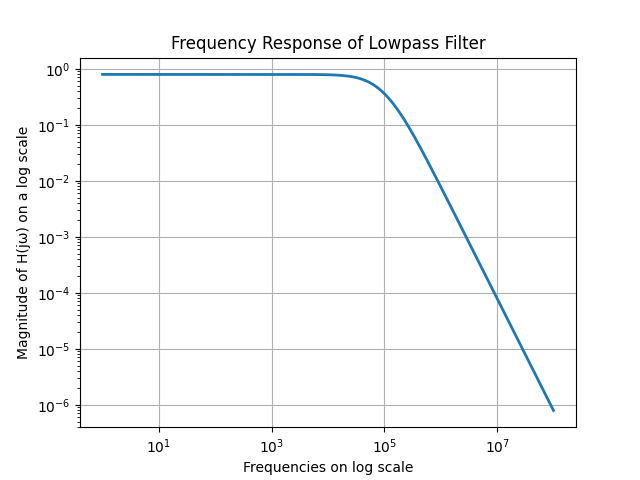
\includegraphics[scale=0.5]{q0.png} 
    \caption{Low Pass Filter's Frequency Response} 	
   \end{figure} 
   
 
\section{The Assignment}  
\subsection{Question 1: Obtaining The Step Response}
For the same low pass filter, I need to find the step response. The input signal will now be $V_i(s)=1/s$. The \texttt{sp.impulse()} function operates on an LTI function to give the inverse Laplace Transform over the given time interval. Here \texttt{V\_q1[3]} is the unit response in $s$ domain. A challenge is to convert the \texttt{sympy} function to an LTI object. This is done by the function \texttt{convert\_sympy\_to\_lti}. It parses the numerator and denominator polynomial coefficients and \texttt{sp\.lti} returns the transfer function.  
\begin{verbatim}
def convert_sympy_to_lti(symbolic_exprn, s = symbols('s')):
    num, den = simplify(symbolic_exprn).as_numer_denom()
    # expressions in reduced form, 
    then separate numerator and denominator
    # print(num,den)
    p_num_den = poly(num, s), poly(den, s)  # polynomials
    # print(p_num_den)
    c_num_den = [p.all_coeffs() for p in p_num_den]  
    # coefficients
    # elements of c_num_den are <class 'sympy.core.numbers.One'>,
     not float
    l_num, l_den = [lambdify((), c)() for c in c_num_den]  
    # convert to floats
    return sp.lti(l_num, l_den)
\end{verbatim} 
Now to get the time domain response, I need to use \texttt{sp.impulse()}, which works on an LTI object given by the above function. Then I plot the output. 
\begin{verbatim}
conductance_matrix_q1, I_q1, V_q1 = lowpass(10000, 10000,
 1e-9, 1e-9, 1.586, 1/s)
print('Unit Response Vo(s) = {}'.format(V_q1[3]))
# Vo_func = lambdify(s,V_q1[3],'numpy')
t, unit_response_in_t = sp.impulse(convert_sympy_to_lti
   (V_q1[3]), None, np.linspace(0, 0.005, 1000))
plt.plot(t, unit_response_in_t, label='Output')
plt.plot(t,np.ones(1000),'red',label='Input')
plt.xlabel('Time')
plt.ylabel('voltage')
plt.title('Step Response of LPF')
plt.grid()
plt.legend()
plt.show()
\end{verbatim}    

  \begin{figure}[!tbh]
   	\centering
  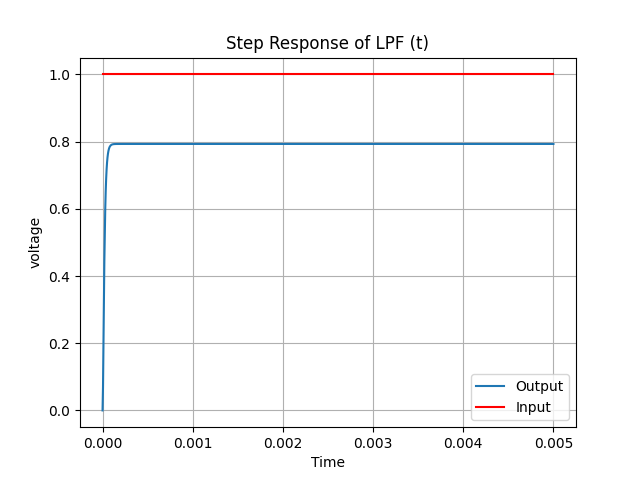
\includegraphics[scale=0.5]{q1.png} 
    \caption{Step Response Of LPF} 	
   \end{figure} 

\subsection{Question 2: Sinusoidal Input Signal}
$$V_i(t)=(\sin(2000\pi t)+\cos(2*10^6\pi t)u(t)$$
This signal is fed to the Low Pass Filter. I start by obtaining the transfer function from the introductory part, then perform the \texttt{sp.lsim} magic that processes the arguments - transfer function  and time domain input over the given interval. The code:
\begin{verbatim}
t = np.linspace(0,0.005,100000)
Vi_t_q2 = np.sin(2000*np.pi*t) + np.cos(2e6*np.pi*t)
transfer_func_lowpass = convert_sympy_to_lti(Vo)  
# reference to Question 0
t,Vo_t_q2,_ = sp.lsim(transfer_func_lowpass, Vi_t_q2, t)

plt.plot(t,Vi_t_q2,'red', label='input')
plt.plot(t, Vo_t_q2, label='output')
plt.xlabel('time')
plt.ylabel('voltage')
plt.title('LPF Input - Output')
plt.legend()
plt.grid()
plt.show()
\end{verbatim}

In the plot, Figure 4, it can be seen that the high frequency signal is filtered out. 

  \begin{figure}[!tbh]
   	\centering
  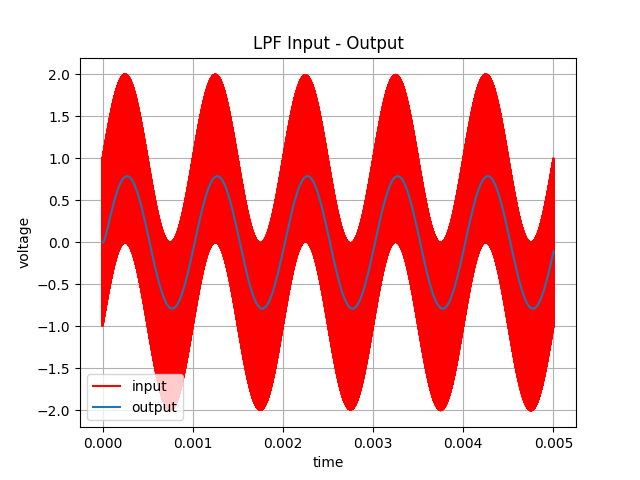
\includegraphics[scale=0.5]{q2.png} 
    \caption{Question 2} 	
   \end{figure} 

\subsection{Question 3: High Pass Filter}
Now that we analysed the working of a low pass filter, its time to study the high pass filter. An active HPF circuit is shown in Figure 5. $R_1 = R_3 = 10kΩ, C_1 = C_2 = 1nF$, and $G = 1.586$
See Figure 5. 
  \begin{figure}[!tbh]
   	\centering
  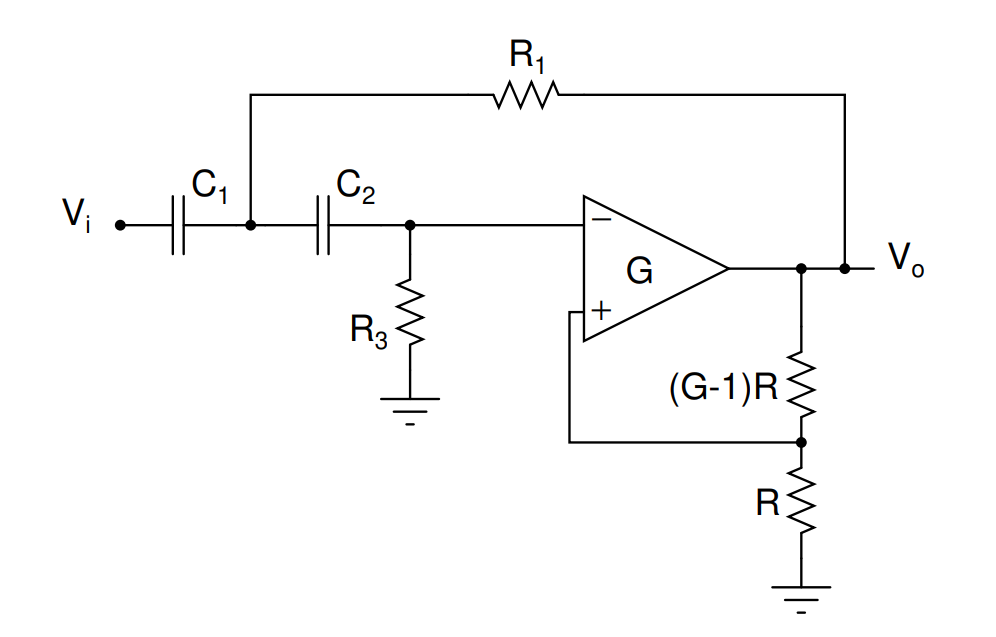
\includegraphics[scale=0.5]{hpfckt.png} 
    \caption{High Pass Filter} 	
   \end{figure} 

Start by defining a \texttt{highpass} function that solves the opamp circuit and returns the voltages at each node. 

\begin{verbatim}
def highpass(R1, R3, C1, C2, G, Vi):
    # A*V = b
    A = Matrix([[0, -1, 0, 1 / G], [G, -G, 0, -1], 
       [s * C2 + 1 / R3, 0, -s * C2, 0], 
       [-C2 / C1, 0, 1 + C2 / C1 + 1 / (s * C1 * R1),
        -1 / (s * C1 * R1)]])
    b = Matrix([0, 0, 0, Vi])
    V = A.inv() * b
    return (A, V, b)
\end{verbatim}

The HPF is characterized by its transfer function - the output voltage signal at $V_i(s)=1$. \texttt{labmdify} converts the $s$ symbolic function to a Python function. Then I plot it. 

\begin{verbatim}
conductance_matrix_q3, variable_voltages_q3, b_q3 = 
   highpass(1e4, 1e4, 1e-9, 1e-9, 1.586,1)
transfer_func_highpass = lambdify(s, variable_voltages_q3[3],
   'numpy')  # output at Vi(s) = 1
plt.loglog(ww, abs(transfer_func_highpass(ss)), lw=2)
plt.xlabel('frequencies')
plt.ylabel('|H(jw)|')
plt.title('Transfer Function Magnitude')
plt.grid()
plt.show()
\end{verbatim}  

  \begin{figure}[!tbh]
   	\centering
  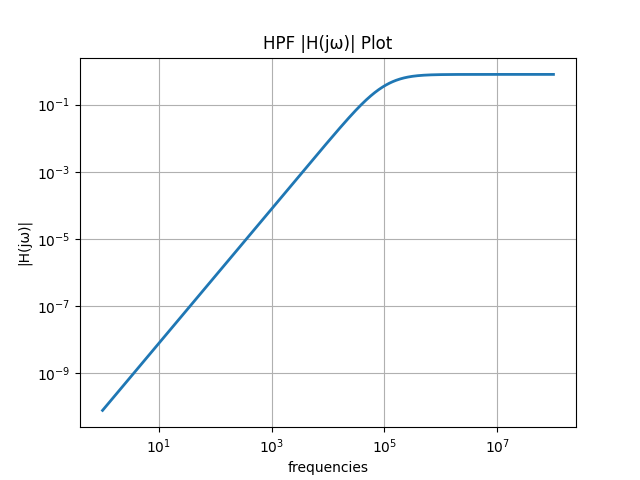
\includegraphics[scale=0.5]{q3.png} 
    \caption{Transfer Function of High Pass Filter} 	
   \end{figure} 


\subsection{Question 4: Damped Sinusoid}
To analyse the response of the HPF to a damped sinusoid, I study its response to first, a low frequency input, then a high frequency. \\
Again, \texttt{sp.lsim} finds the time domain output. The two signals are $$V1_i(t)=e^{-5t}\cos(20\pi t)$$
$$V2_i(t)=e^{-50000t}\cos(2*10^8\pi t)$$

\begin{verbatim}
damping_fac = 5
t1 = np.linspace(0,1,1000)
V1_q4 = np.exp(-damping_fac*t1)*np.cos(20*np.pi*t1)
H = convert_sympy_to_lti(variable_voltages_q3[3])
t1,Vo1_q4,_ = sp.lsim(H, V1_q4,t1)

plt.plot(t1,V1_q4,label='input')
plt.plot(t1,Vo1_q4,label='output')
plt.xlabel('time')
plt.ylabel('voltage')
plt.title('Low Frequency Input')
plt.legend()
plt.grid()
plt.show()
\end{verbatim}

One can expect this function to not pass through, the plot is seen in Figure 7.

  \begin{figure}[!tbh]
   	\centering
  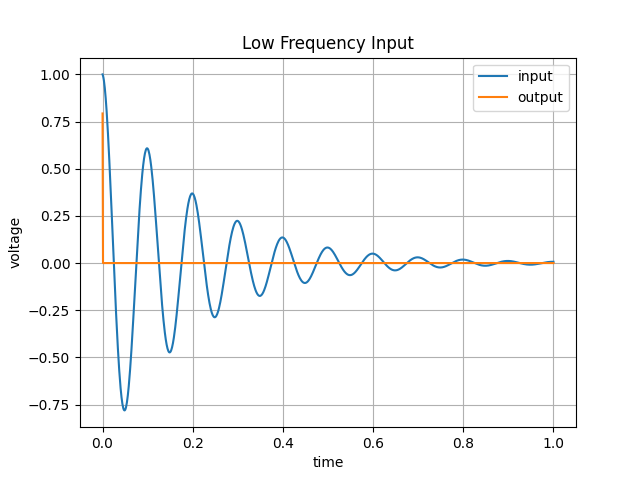
\includegraphics[scale=0.5]{q4.png} 
    \caption{Low Frequency Damped Input} 	
   \end{figure} 
   
Next, a high frequency damped input. Since I have used a frequency higher than the pole frequency, this should pass through the filter. See Figure 8.
\begin{verbatim}
damping_fac = 50000
t2 = np.linspace(0,0.0001,1000)
V2_q4 = np.exp(-damping_fac*t2)*np.cos(2e8*np.pi*t2)
t2,Vo2_q4,_ = sp.lsim(H, V2_q4,t2)

plt.plot(t2,V2_q4,label='input')
plt.plot(t2,Vo2_q4,label='output')
plt.xlabel('time')
plt.ylabel('voltage')
plt.title('High Frequency Input')
plt.legend()
plt.grid()
plt.show()
\end{verbatim} 

  \begin{figure}[!tbh]
   	\centering
  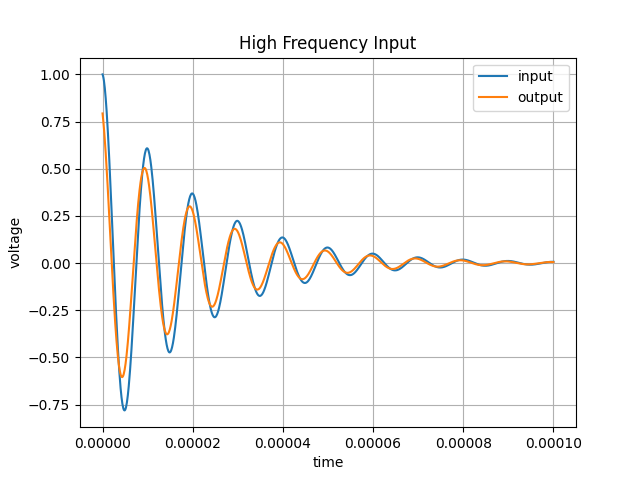
\includegraphics[scale=0.5]{q4-2.png} 
    \caption{High Frequency Damped Input} 	
   \end{figure} 
   
\subsection{Question 5: Unit Step Response}
Unit step at the input is $V_i(s)=1/s$ which is given to \texttt{highpass} to obtain the frequency domain sympy output. This is converted to time domain by \texttt{sp.impulse}. The plot is Figure 9.   

\begin{verbatim}
conductance_matrix_q5, variable_voltages_q5, V_q5 = 
highpass(10000, 10000, 1e-9, 1e-9, 1.586, 1/s)
print('Unit Response Vo(s) = {}'.format(V_q1[3]))
# Vo_func = lambdify(s,V_q1[3],'numpy')
t, unit_response_hpf = sp.impulse(convert_sympy_to_lti
(variable_voltages_q5[3]), None, np.linspace(0, 0.001, 10000))
plt.plot(t, unit_response_hpf, label='Output')
plt.plot(t,np.ones(len(t)),'red',label='Input')
plt.xlabel('Time')
plt.ylabel('voltages')
plt.title('Step Response of HPF')
plt.legend()
plt.grid()
plt.show()
\end{verbatim}

The zero output is because the capacitors will quickly ($< 0.1 ms$) block DC and no signal will reach the opamp. 

  \begin{figure}[!tbh]
   	\centering
  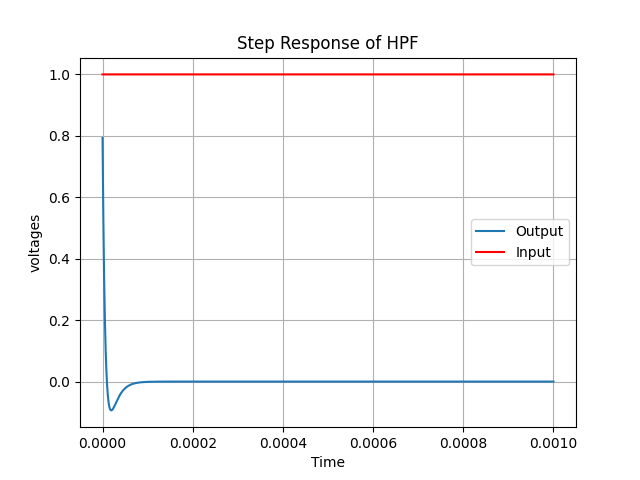
\includegraphics[scale=0.5]{q5.png} 
    \caption{HPF Unit Step Response}
   \end{figure} 

\section{Conclusion}
The goal that I started the assignment with, I now seen to have been accomplished. Symbolic algebra is implemented in Python by the \texttt{sympy} library. Combining the use of symbols in functions to analyse filters and their transfer functions is what most of the assignment was about. I also observed the behavior of these filters for different frequencies of input. 


\end{document}



 